\documentclass[12pt]{article}
%Gummi|065|=)
\usepackage{amsmath, amsfonts, amssymb}
\usepackage[margin=0.5in]{geometry}
\usepackage{xcolor}
\usepackage{graphicx}
\usepackage{ifthen}

\usepackage{pifont}
\usepackage{amsmath}

\newcommand{\off}[1]{}
\DeclareMathSizes{20}{30}{20}{18}

\newcommand{\two }{\sqrt[3]{2}}
\newcommand{\four}{\sqrt[3]{4}}
\newcommand{\red}{\begin{tikz}[scale=0.25]
\draw[fill=red, color=red] (0,0)--(1,0)--(1,1)--(0,1)--cycle;\end{tikz}}
\newcommand{\blue}{\begin{tikz}[scale=0.25]
\draw[fill=blue, color=blue] (0,0)--(1,0)--(1,1)--(0,1)--cycle;\end{tikz}}
\newcommand{\green}{\begin{tikz}[scale=0.25]
\draw[fill=green, color=green] (0,0)--(1,0)--(1,1)--(0,1)--cycle;\end{tikz}}

\newcommand{\sq}[3]{\draw[#3] (#1,#2)--(#1+1,#2)--(#1+1,#2+1)--(#1,#2+1)--cycle;}
\newcommand{\linebrk}{----------------------------------------------------------------------------------------------------------------------------------}


\usepackage{tikz}

\newcommand{\susy}{{\bf Q}}
\newcommand{\RV}{{\text{R}_\text{V}}}

\title{Tutorial : Ping-Pong Lemma}
\date{}
\begin{document}

\fontfamily{qag}\selectfont \fontsize{12.5}{15}\selectfont

\maketitle

\noindent Half of these projects start by a conjectured relationship between two theorems.  And it's not always correct.  Today's pair is:
\begin{itemize}
\item Ping-Pong Lemma
\item Sum-Product Theorem
\end{itemize}
I \textit{think} that's correct. Let's state these results and being the long journey of connecting these thing to ``real life". \\ \\
\textbf{\#1 Ping-Pong Lemma} I was able to find two examples of Ping-Pong Lemma having to with group matrices over the integers $\mathbb{Z}$ we can have
\begin{itemize}
\item Banach-Tarski paradox
\item Establishing free groups
\end{itemize}  
Here's a proposition:
\begin{quotation} \noindent This is a Free group on two generators (no relations)
$$ \left\langle \left(\begin{array}{cc} 1 & 2 \\ 0 & 1 \end{array} \right),
\left(\begin{array}{cc} 1 & 0 \\ 2 & 1 \end{array} \right) \right\rangle \subseteq SL_2(\mathbb{Z}) $$
Proof: use the ping-pong Lemma.  Another example I found from Sarnak\footnote{\texttt{http://web.math.princeton.edu/sarnak/NotesOnThinGroups.pdf}} 
$$ \left\langle \left(\begin{array}{cccr} 0 & 0 & 0 & -1 \\
1 & 0 & 0 & -1 \\
0 & 1 & 0 & -1 \\
0 & 0 & 1 & -1 \end{array} \right),
\left(\begin{array}{cccr}
1 & 0 & 0 & -5 \\
0 & 1 & 0 & -5 \\
0 & 0 & 1 & -5 \\ 
 0 & 0 & 0 & -5\end{array} \right)
\right\rangle \subseteq SL_4(\mathbb{Z}) $$
and these play generalized Ping-Pong.  The reason we like the free group $F_2$
is becuase it's one of the few discrete groups we can understand. And I don't even think that's true, because if $A,B \in SO(3)$ that group is compact and we can measure:
$$ \phi: \langle A,B \rangle \to SO(3) $$
we'd have that $\overline{\langle A,B \rangle} \subseteq SO(3)$ is a \textbf{dense} subgroup, so we can try to quantify (by whatever means we have availble) how quickly this is mixing.
\end{quotation}
In another direction we have the Banach-Tarski paradox.  The groups used to contruct the paradox seem related to the Pythagorean theorem\footnote{https://stanford.box.com/shared/static/wesg27648yqomf4ar3mkmfwf89ptzqj4.pdf} He will use:
\begin{quotation}\noindent This group is free:
$$  \left\langle \left( \begin{array}{ccc} \frac{1}{3} & +\frac{2 \sqrt{3}}{3} & 0 \\
-\frac{2 \sqrt{3}}{3} &  \frac{1}{3} &  0 \\
0 & 0 & 1
\end{array}\right) , 
\left( \begin{array}{ccc}
1 & 0 & 0  \\
0 &  \frac{1}{3} & +\frac{\sqrt{8}}{3}  \\
0 & -\frac{ \sqrt{8}}{3} &  \frac{1}{3}  \\
\end{array}\right) 
\right\rangle \subseteq SO_3(\mathbb{R})$$
This group is related to the right triangle with side lengths $1$ and $\sqrt{8}$\\
\begin{center}
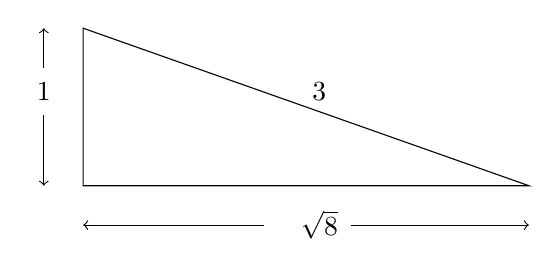
\begin{tikzpicture}[scale=2]
\draw (0,0)--(2.83,0)--(0,1)--cycle;
\node at (-0.25,0.6) {$1$};
\draw[->] (-0.25,0.45)--(-0.25,0);
\draw[->]  (-0.25,0.75)--(-0.25,1);

\node at (1.5, 0.6) {$3$};

\node at (1.5,-0.25) {$\sqrt{8}$};
\draw[->] ( 1.15,-0.25)--(0,-0.25);
\draw[->] (1.7, -0.25)--(2.83, -0.25);

\end{tikzpicture} \\
\end{center}
This tringle is oriented in various ways in three dimensional space.
\end{quotation}
Therefore\dots without stating the ping-pong Lemma we can imagine such a thing could be useful!  Now for the statement:
\begin{quotation}\noindent 
\textbf{\color{red!50!white}Ping-Ping Lemma} {\color{green!50!blue} Let $G$ be a group acting on a set $X$.  Let $H_1, H_2$ be sub-groups and suppose we can find subsets $X_1, X_2 \subseteq X$ subset that we observe
$$
\big[ g \in H_1 \to g(X_2) \subseteq X_1 \big] \text{ and }
\big[ g \in H_2 \to g(X_1) \subseteq X_2 \big] $$   
then our subgroup is free, $\langle H_1, H_2 \rangle = H_1 \ast H_2 \simeq F_2$}.
\end{quotation}
One thing we notice is that ping-pong ``works" (i.e. produces free groups or expander graphs?) only for $3 \times 3$ and not for $2 \times 2$.  Another possiblity is that the group we are studying isn't free (there are relations).  This is not a bad thing, $SL(2, \mathbb{Z})$ is not free, there's a relation:
$$ SL_2\,(\, \mathbb{Z}\,) \simeq \big\langle S, T: S^2 = (ST)^3 = 1 \big\rangle \simeq \big( \mathbb{Z}/2\mathbb{Z} \big) \ast \big( \mathbb{Z}/3\mathbb{Z} \big) $$
and for a general number field, $F$, $SL_2( \mathcal{O}_F)$ for the ring of integers $\mathcal{O}_F$ can be an open problem.  Therefore, we conclude, $SL(2, \mathbb{Z})$ can house rather complicated objects. \\ \\
\textbf{\#2 Sum-Product Theorem} \dots \\ \\
\textbf{\#2 Approximate Groups} \dots \\ \\
\textbf{\#3 Do these two overlap?} \dots \\ \\

\vfill

\begin{thebibliography}{}

\item \dots

\end{thebibliography}



\end{document}